% Suggested LaTeX style template for Masters project report submitted at the
% Department of Computer Science and Technology
%
% Markus Kuhn, May 2022
% (borrowing elements from an earlier template by Steven Hand)

\documentclass[12pt,a4paper,twoside]{report}
% append option ",openright" after "twoside" if you prefer each chapter
% to start on a recto (odd-numbered) page in a double-sided printout

\usepackage[pdfborder={0 0 0}]{hyperref}
\usepackage[vmargin=20mm,hmargin=25mm]{geometry}
\usepackage{graphicx}
\usepackage{parskip}
\usepackage{setspace}
\usepackage{refcount}
\usepackage{upquote}
\usepackage{xcolor}
\usepackage{subcaption}
\usepackage{amsmath}
\usepackage{amssymb}
\usepackage[sort,numbers]{natbib}
\usepackage[capitalise]{cleveref}
\usepackage{adjustbox}
\usepackage{listings}
\usepackage{float}
\usepackage{tabularx}
\usepackage{booktabs}
\usepackage{multirow}
\usepackage{xspace}
\usepackage{tikz}
\usetikzlibrary{arrows,calc,arrows.meta,positioning}

\lstset{
basicstyle=\small\ttfamily,
columns=fullflexible,
breaklines=true,
}

\hypersetup{
    colorlinks,
    linkcolor={blue!50!black},
    citecolor={blue!50!black},
    urlcolor={black}
}

\newif\ifsubmission % Boolean flag for distinguishing submitted/final version

% Change the following lines to your own project title, name, college, course
\title{End-to-End Ontology Learning with Large Language Models}
\author{Chun Yuen Andy Lo}
\date{May 2024}
\newcommand{\candidatenumber}{1234N}
\newcommand{\college}{Christ's College}
\newcommand{\course}{Computer Science Tripos, Part III}
\newcommand{\todo}[1]{\textcolor{red}{TODO: #1}}
\newcommand{\name}{{OLLM}\xspace}
\newcommand{\m}[1]{\mathbf{#1}}
\newcommand{\R}{\mathbb{R}}
\DeclareMathOperator{\nodesim}{NodeSim}

\hyphenpenalty=0

% Select which version this is:
% For the (anonymous) submission (without your name or acknowledgements)
% uncomment the following line (or let the makefile do this for you)
% \submissiontrue
% For the final version (with your name) leave the above commented.

\begin{document}

%TC:ignore 
\begin{sffamily} % use a sans-serif font for the pro-forma cover sheet

    \begin{titlepage}
        \makeatletter

        % University logo with shield hanging in left margin
        \hspace*{-14mm}\includegraphics[width=65mm]{logo-dcst-colour.pdf}

        \ifsubmission

            % submission proforma cover page for blind marking
            \begin{Large}
                \vspace{20mm}
                Research project report title page

                \vspace{35mm}
                Candidate \candidatenumber

                \vspace{42mm}
                \textsl{``\@title''}

            \end{Large}

        \else

            % regular cover page
            \begin{center}
                \Huge
                \vspace{\fill}

                \@title
                \vspace{\fill}

                \@author
                \vspace{10mm}

                \Large
                \college
                \vspace{\fill}

                \@date
                \vspace{\fill}

            \end{center}

        \fi

        \vspace{\fill}
        \begin{center}
            Submitted in partial fulfillment of the requirements for the\\
            \course
        \end{center}

        \makeatother
    \end{titlepage}

    \newpage

    Total page count: \pageref{lastpage}

    % calculate number of pages from
    % \label{firstcontentpage} to \label{lastcontentpage} inclusive
    \makeatletter
    \@tempcnta=\getpagerefnumber{lastcontentpage}\relax%
    \advance\@tempcnta by -\getpagerefnumber{firstcontentpage}%
    \advance\@tempcnta by 1%
    \xdef\contentpages{\the\@tempcnta}%
    \makeatother

    Main chapters (excluding front-matter, references and appendix):
    \contentpages~pages
    (pp~\pageref{firstcontentpage}--\pageref{lastcontentpage})

    Main chapters word count: 10000\footnote{Computed with \texttt{texcount}.}

\end{sffamily}

\vspace{\fill}
\onehalfspacing
\makeatletter
\textbf{\Huge Declaration}
\vspace{40pt}

\ifsubmission
    I, [Blind candidate number], being a candidate for Part III of the Computer Science Tripos, hereby declare that this project report and the work described in it are my own work, unaided except as may be specified below, and that the project report does not contain material that has already been used to any substantial extent for a comparable purpose. The project required the use of AI-assisted platform GitHub Copilot in chapter 3 and 4, and such use is acknowledged in the text. I am content for my project report to be made available to the students and staff of the University.

    \bigskip
    \textbf{Date:} \today
\else
    I, \@author\ of \college, being a candidate for Part III of the Computer Science Tripos, hereby declare that this project report and the work described in it are my own work, unaided except as may be specified below, and that the project report does not contain material that has already been used to any substantial extent for a comparable purpose. The project required the use of AI-assisted platform GitHub Copilot in chapter 3 and 4, and such use is acknowledged in the text. I am content for my project report to be made available to the students and staff of the University.

    \bigskip
    \textbf{Signed:} \@author

    \bigskip
    \textbf{Date:} \today
\fi
\vspace{\fill}
\makeatother

\chapter*{Abstract}

Ontologies are useful for automatic machine processing as they represent knowledge in a structured format. Yet, constructing ontologies requires substantial manual effort. To automate part of this process, large language models (LLMs) have been applied to solve various subtasks of ontology learning. However, this partial ontology learning does not capture the interactions between subtasks.
We address this gap by introducing \name, a general and scalable method for solving the \emph{full} task of building an ontology from scratch.
Rather than focusing on subtasks, like individual relations between entities, we model entire subcomponents of the target ontology by finetuning an LLM with a custom regulariser that reduces overfitting on high-frequency concepts. We introduce a novel suite of metrics for evaluating the quality of the generated ontology by measuring its semantic and structural similarity to the ground truth. Our metrics stem from modern deep learning evaluation techniques, but make fewer assumptions about the ontologies than standard ontology metrics.
Our results on Wikipedia show that \name outperforms subtask composition methods, producing more semantically accurate ontologies while maintaining structural integrity. We further demonstrate that our model can be effectively adapted to a new domain, like arXiv, needing only a small number of training examples.

\ifsubmission\else
    % not included in submission for blind marking:

    \chapter*{Acknowledgements}

    This project would not have been possible without the wonderful
    support of \ldots [optional]

\fi
\cleardoublepage % preserve page numbers after missing acknowledgements

\tableofcontents
%\listoffigures
%\listoftables
%TC:endignore 

\chapter{Introduction}  \label{chap:introduction}

\label{firstcontentpage} % start page count here

An ontology is a formal and structural way of representing domain-specific concepts and their relations~\cite{gruber1995toward}.
They can be simple (e.g., Wikipedia categories) consisting of \emph{concepts} and only a small number of types of \emph{taxonomic relations} (e.g., \emph{is-a} relationships), or they can be complex (e.g., Schema.org) consisting of axioms or many types of relations. For example, a simple ontology for programming languages might be:

\begin{figure}[H]
    \centering
    \sffamily
    \newcommand{\dist}{1.5cm}
    \begin{tikzpicture}[>=latex]
        \node[rectangle] (dynamically-typed) {Dynamically-typed language};
        \node[rectangle] (python) at ($(dynamically-typed) + (-\dist, -\dist)$) {Python};
        \node[rectangle] (js) at ($(dynamically-typed) + (\dist, -\dist)$) {JavaScript};
        \draw[->] (dynamically-typed) -- (python);
        \draw[->] (dynamically-typed) -- (js);
    \end{tikzpicture}
\end{figure}

It has three concepts and two relations, representing the knowledge that Python and JavaScript are dynamically-typed languages. A more complex ontology might contain axioms too, for example, ``all programming languages are either dynamically or statically typed''.
In this project, we focus on ontologies with only concepts and taxonomic relations. Compared to typical deep learning models, which represent knowledge implicitly in its weights, ontologies capture knowledge in a structured and explicit manner, making them reliable, easy to edit and human-interpretable. Such benefits of ontologies have led to their wide adoption in practice. For example, Wikipedia categories have been used for entity ranking~\cite{vercoustre2008using} and information retrieval~\cite{sorg2012exploiting}, or Schema.org~\cite{Schema.org_2011} is a core component of the Semantic Web~\cite{antoniou2004semantic} initiative.

While ontologies are useful, building ontologies often requires substantial manual effort. Ontology learning (OL) is the study of automating the construction of high-quality ontologies at scale. For a simple ontology, this amounts to discovering the concepts and taxonomic relations, usually based on a source corpus. In this project we aim to develop domain-independent methods for OL that are scalable and produce better ontologies.

\section{Project goals}

Traditionally, OL is viewed as a composition of subtasks~\cite{asim2018survey}, such as concept discovery and relation extraction. In particular, prior works have demonstrated that state-of-the-art large language models (LLMs) can solve such subtasks effectively~\cite{babaei2023llms4ol}. While studying subtasks permits fine-grained analysis and evaluation, it does not directly indicate the subsequent impact on the quality of the final ontology. Moreover, there is potential room for improvement by combining several subtasks into one, such as by modelling concepts and relations in conjunction. In this project, we instead develop and evaluate methods that construct ontologies in an end-to-end fashion to answer the following research questions:
\begin{enumerate}
    \item How can we leverage LLMs' knowledge base to build ontologies from scratch?
    \item Does our method scale efficiently to practical problem sizes?
    \item How well does our method generalise to new domains?
\end{enumerate}

\section{Achievements}

\begin{figure}[t]
    \centering
    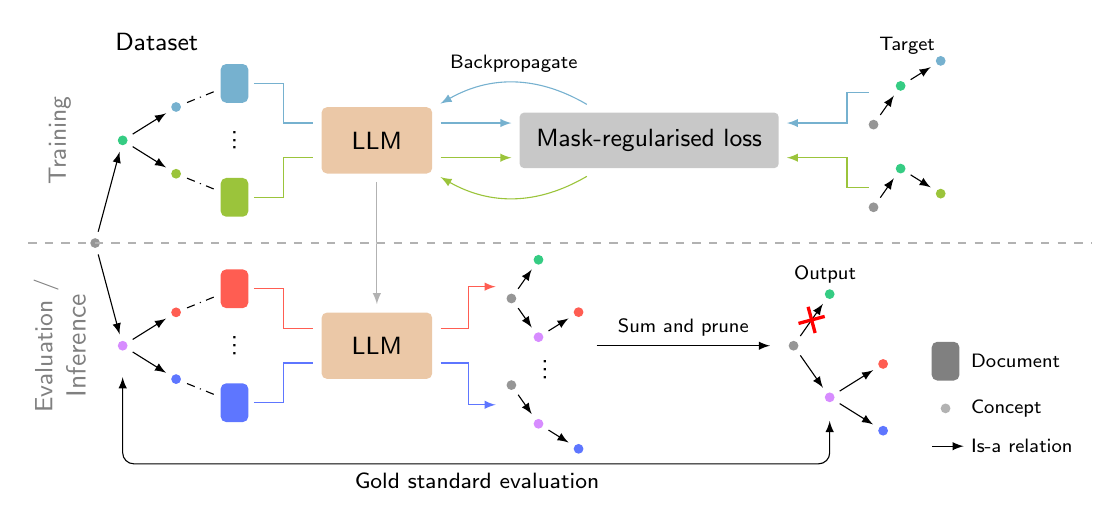
\begin{tikzpicture}
        [
            >=latex,
            doc/.style={
                    rectangle,
                    rounded corners=2pt,
                    minimum width=10pt,
                    minimum height=14pt,
                    outer sep=2pt,
                },
            llm/.style={
                    rectangle,
                    rounded corners=2pt,
                    fill={black!20},
                    minimum width=40pt,
                    minimum height=24pt,
                    outer sep=3pt,
                },
            concept/.style={
                    circle,
                    fill={black!30},
                    inner sep=1.25pt,
                    outer sep=2.5pt,
                },
            every node/.append style={font=\sffamily},
            pics/.cd,
            % Marque croix en diagonale
            Cross/.style args={#1 and #2}{%
                    code = {%
                            \draw[#2,rotate=45,scale=1.4,very thick]
                            (0,#1 pt) -- (0,-#1 pt) ;
                            \draw[#2,rotate=-45,scale=1.4,very thick]
                            (0,#1 pt) -- (0,-#1 pt) ;
                        }
                },
            Cross/.default={2.5 and gray!25!black},
        ]
        \newcommand{\nodeDist}{0.8}
        \newcommand{\nodeDistShort}{0.6}
        \newcommand{\angleA}{15}
        \newcommand{\angleB}{58}
        \definecolor{c0}{RGB}{150, 150, 150}
        \definecolor{c1}{RGB}{255, 93, 82}
        \definecolor{c2}{RGB}{94, 118, 255}
        \definecolor{c3}{RGB}{118, 177, 207}
        \definecolor{c4}{RGB}{215, 140, 255}
        \definecolor{c5}{RGB}{155, 196, 59}
        \definecolor{c6}{RGB}{53, 204, 131}
        \definecolor{llmcolor}{RGB}{235, 200, 167}
        \definecolor{losscolor}{RGB}{200, 200, 200}

        % PART A: Ontology
        \node[concept,color=c0] (root) {};
        \node[concept,color=c4] (l1) at ($(root) + ({-90+\angleA}:{\nodeDist+0.55})$) {};
        \node[concept,color=c6] (l2) at ($(root) + ({90-\angleA}:{\nodeDist+0.55})$) {};
        \node[concept,color=c1] (l11) at ($(l1) + ({90-\angleB}:{\nodeDist})$) {};
        \node[concept,color=c2] (l12) at ($(l1) + ({-90+\angleB}:{\nodeDist})$) {};
        \node[concept,color=c3] (l21) at ($(l2) + ({90-\angleB}:{\nodeDist})$) {};
        \node[concept,color=c5] (l22) at ($(l2) + ({-90+\angleB}:{\nodeDist})$) {};
        % \node[concept] (l1) at ($(root) + ({180+\angleA}:{\nodeDist})$) {};
        % \node[concept] (l2) at ($(root) + ({-\angleA}:{\nodeDist})$) {};
        % \node[concept] (l11) at ($(l1) + ({180+\angleB}:{\nodeDist})$) {};
        % \node[concept] (l12) at ($(l1) + ({-\angleB}:{\nodeDist})$) {};
        % \node[concept] (l21) at ($(l2) + ({180+\angleB}:{\nodeDist})$) {};
        % \node[concept] (l22) at ($(l2) + ({-\angleB}:{\nodeDist})$) {};
        \draw[->] (root) -- (l1);
        \draw[->] (root) -- (l2);
        \draw[->] (l1) -- (l11);
        \draw[->] (l1) -- (l12);
        \draw[->] (l2) -- (l21);
        \draw[->] (l2) -- (l22);

        \node[anchor=west,inner sep=0,align=left] (caption) at ($(root.west) + (0.4, 2.55)$) {\small Dataset};

        \newcommand{\docSpace}{0.66}
        \node[doc,fill=c1] (doc1) at ($(l11) + ({90-\angleB-10}:{\nodeDist})$) {};
        \node[doc,fill=c2] (doc2) at ($(l12) + ({-90+\angleB+10}:{\nodeDist})$) {};
        \node[doc,fill=c3] (doc3) at ($(l21) + ({90-\angleB-10}:{\nodeDist})$) {};
        % \node[doc,fill=c4] (doc4) at ($(l11) + (\docSpace, -1.5)$) {};
        \node[doc,fill=c5] (doc7) at ($(l22) + ({-90+\angleB+10}:{\nodeDist})$) {};
        \node[doc,rotate=90] (doc5) at ($(doc1)!0.5!(doc2)$) {...};
        \node[doc,rotate=90] (doc6) at ($(doc3)!0.5!(doc7)$) {...};
        \draw[dashdotted] (l11) to (doc1);
        \draw[dashdotted] (l12) to (doc2);
        \draw[dashdotted] (l21) to (doc3);
        \draw[dashdotted] (l22) to (doc7);
        % \draw[dashdotted,bend right] (l1) to (doc4);

        % line to separate the ontology into train and test
        % \draw[dashed] ($(root) + (0, 0.4)$) -- ($(root) + (0, -2.6)$);
        % \node at ($(root) + (1.1, -0.1)$) {Train};
        % \node at ($(root) + (-1.1, -0.1)$) {Test};

        % \draw[dashed] ($(root) + (-0.4, 0)$) -- ($(root) + (2.0, 0)$);
        % \node[anchor=west,inner sep=0] at ($(root.west) + (0, 1.1)$) {\small Train};
        % \node[anchor=west,inner sep=0] at ($(root.west) + (0, -1.5)$) {\small Test};

        % PART B: Training
        \newcommand{\vertSpace}{0.22}
        \newcommand{\trainSpace}{0.7}
        % \node[doc,fill=c3] (input) at ($(doc3) + (1.0, 0)$) {};
        % \node[doc,fill=c5] (inputp) at ($(doc7) + (1.0, 0)$) {};

        \node[llm,anchor=west,fill=llmcolor] (llm) at ($(doc3)!0.5!(doc7) + (1, 0)$) {\small LLM};
        \node[anchor=west,align=center,rounded corners=1.5pt,outer sep=3pt,inner sep=6pt,fill=losscolor] (loss) at ($(llm.east) + (\trainSpace + 0.2, 0)$) {\small Mask-regularised loss};

        \begin{scope}[local bounding box=target1,shift={($(loss.east) + (1.1, 0.2)$)},outer sep=3pt]
            \node[concept,color=c0] (sgRoot) {};
            \node[concept,color=c6] (sg2) at ($(sgRoot) + ({90-\angleA-20}:{\nodeDistShort})$) {};
            \node[concept,color=c3] (sg21) at ($(sg2) + ({90-\angleB}:{\nodeDistShort})$) {};
            \draw[->] (sgRoot) -- (sg2);
            \draw[->] (sg2) -- (sg21);
        \end{scope}

        \begin{scope}[local bounding box=target2,shift={($(loss.east) + (1.1, -0.85)$)},outer sep=3pt]
            \node[concept,color=c0] (sgRoot) {};
            \node[concept,color=c6] (sg2) at ($(sgRoot) + ({90-\angleA-20}:{\nodeDistShort})$) {};
            \node[concept,color=c5] (sg22) at ($(sg2) + ({-90+\angleB}:{\nodeDistShort})$) {};
            \draw[->] (sgRoot) -- (sg2);
            \draw[->] (sg2) -- (sg22);
        \end{scope}

        \coordinate (out) at ($(llm.west) + (0, \vertSpace)$);
        \draw[color=c3] (doc3) -| ($(doc3.east)!0.5!(out)$) |- (out);
        \draw[->,color=c3] ($(llm.east) + (0, \vertSpace)$) -- ($(loss.west) + (0, \vertSpace)$);

        \coordinate (out) at ($(llm.west) + (0, -\vertSpace)$);
        \draw[color=c5] (doc7) -| ($(doc7.east)!0.5!(out)$) |- (out);
        \draw[->,color=c5] ($(llm.east) + (0, -\vertSpace)$) -- ($(loss.west) + (0, -\vertSpace)$);

        \coordinate (out) at ($(loss.east) + (0, \vertSpace)$);
        \draw[->,color=c3] (target1) -| ($(target1)!0.5!(out)$) |- (out);
        \coordinate (out) at ($(loss.east) + (0, -\vertSpace)$);
        \draw[->,color=c5] (target2) -| ($(target2)!0.5!(out)$) |- (out);
        \draw[->,bend right,color=c3] (loss) to node [midway,above,align=center,color=black] {\scriptsize Backpropagate} (llm);
        \draw[->,bend left,color=c5] (loss) to (llm);
        \node at ($(target1) + (0, 0.6)$) {\scriptsize Target};

        % PART C: Inference
        \node[llm,anchor=west,fill=llmcolor] (llm1) at ($(doc1)!0.5!(doc2) + (1.0, 0)$) {\small LLM};
        % \node[doc,fill=c1,anchor=east] (input1) at ($(llm1.west) + (-\trainSpace, 0.8)$) {};

        \begin{scope}[local bounding box=sg1,shift={($(llm1.east) + (\trainSpace + 0.2, 0.6)$)}]
            \node[concept,color=c0] (sgRoot1) {};
            \node[concept,color=c4] (sg11) at ($(sgRoot1) + ({-90+\angleA+20}:{\nodeDistShort})$) {};
            \node[concept,color=c6] (sg12) at ($(sgRoot1) + ({90-\angleA-20}:{\nodeDistShort})$) {};
            \node[concept,color=c1] (sg112) at ($(sg11) + ({90-\angleB}:{\nodeDistShort})$) {};
            \draw[->] (sgRoot1) -- (sg12);
            \draw[->] (sgRoot1) -- (sg11);
            \draw[->] (sg11) -- (sg112);
        \end{scope}

        \begin{scope}[local bounding box=sg2,shift={($(llm1.east) + (\trainSpace + 0.2, -0.5)$)}]
            \node[concept,color=c0] (sgRoot2) {};
            \node[concept,color=c4] (sg21) at ($(sgRoot2) + ({-90+\angleA+20}:{\nodeDistShort})$) {};
            \node[concept,color=c2] (sg211) at ($(sg21) + ({-90+\angleB}:{\nodeDistShort})$) {};
            \draw[->] (sgRoot2) -- (sg21);
            \draw[->] (sg21) -- (sg211);
        \end{scope}


        % \node (dots) at ($(input1)!0.5!(input2)$) {...};
        % \node (dots2) at ($(dots) + (4.0, 0)$) {...};
        \node[rotate=90] at ($(sg1)!0.5!(sg2) + (0, -0.15)$) {...};
        \draw[color=c1] (doc1) -| ($(doc1.east)!0.5!(llm1.west)$) |- ($(llm1.west) + (0, \vertSpace)$);
        \coordinate (out1) at ($(llm1.east) + (\trainSpace, 0.75)$);
        \draw[->,color=c1] ($(llm1.east) + (0, \vertSpace)$) -| ($(llm1.east)!0.5!(out1)$) |- (out1);
        \draw[color=c2] (doc2) -| ($(doc2.east)!0.5!(llm1.west)$) |- ($(llm1.west) + (0, -\vertSpace)$);
        \coordinate (out2) at ($(llm1.east) + (\trainSpace, -0.75)$);
        \draw[->,color=c2] ($(llm1.east) + (0, -\vertSpace)$) -| ($(llm1.east)!0.5!(out2)$) |- (out2);


        % \node[doc,fill=c1] (input1) at ($(input) + (0, -2.0)$) {};
        % \node[llm] (llm1) at ($(input1) + (\trainSpace, 0)$) {LLM};
        % \node[concept] (sgRoot1) at ($(llm1) + (\trainSpace + 0.8, 0.6)$) {};
        % \node[concept] (sg11) at ($(sgRoot1) + ({180+\angleA}:{\nodeDist})$) {};
        % \node[concept] (sg12) at ($(sgRoot1) + ({-\angleA}:{\nodeDist})$) {};
        % \node[concept] (sg111) at ($(sg11) + ({180+\angleB}:{\nodeDist})$) {};
        % \draw[->] (input1) -- (llm1);
        % \draw[->] (llm1) -- ($(llm1) + (\trainSpace-0.25, 0)$);

        % \node[doc,fill=c2] (input2) at ($(input1) + (0, -1.7)$) {};
        % \node[llm] (llm2) at ($(input2) + (\trainSpace, 0)$) {LLM};
        % \node[concept] (sgRoot2) at ($(llm2) + (\trainSpace + 0.8, 0.6)$) {};
        % \node[concept] (sg21) at ($(sgRoot2) + ({180+\angleA}:{\nodeDist})$) {};
        % \node[concept] (sg212) at ($(sg21) + ({-\angleB}:{\nodeDist})$) {};
        % \draw[->] (input2) -- (llm2);
        % \draw[->] (llm2) -- ($(llm2) + (\trainSpace-0.25, 0)$);

        \node[concept,color=c0] (testOutRoot) at ($(doc1)!0.5!(doc2) + (7.1, 0.0)$) {};
        \node[concept,color=c4] (testOut1) at ($(testOutRoot) + ({-90+\angleA+20}:{\nodeDist})$) {};
        \node[concept,color=c2] (testOut11) at ($(testOut1) + ({-90+\angleB}:{\nodeDist})$) {};
        \node[concept,color=c1] (testOut12) at ($(testOut1) + ({90-\angleB}:{\nodeDist})$) {};
        \node[concept,color=c6] (testOut2) at ($(testOutRoot) + ({90-\angleA-20}:{\nodeDist})$) {};
        \node at ($(testOutRoot) + (0.4, 0.9)$) {\scriptsize Output};
        \draw[->] (testOutRoot) -- (testOut1);
        \draw[->] (testOut1) -- (testOut11);
        \draw[->] (testOut1) -- (testOut12);
        \draw[->] (testOutRoot) -- pic[midway,-,rotate=60] {Cross={3.5 and red}} (testOut2);
        \draw[->] ($(doc1)!0.5!(doc2) + (4.6, 0)$) -- node [midway,above,align=center] {\scriptsize Sum and prune} ($(doc1)!0.5!(doc2) + (6.8, 0)$);

        % PART D: Evaluation
        \coordinate (start) at ($(l1) + (0, -0.4)$);
        \coordinate (inter) at ($(start) + (4.5, -1.1)$);
        \coordinate (end) at ($(testOut1) + (0, -0.3)$);
        \draw[<->,rounded corners] (start) |- (inter) -| (end);
        \node[below] at (inter) {\footnotesize Gold standard evaluation};

        % Draw a separation line between Part B and Part C
        \draw[color={black!30},dashed] ($(root) + (-0.85, 0)$) -- ($(root) + (12.65, 0)$);
        % Caption Part B
        \node[color={black!50},inner sep=0,rotate=90] at ($(l2) + (-0.8, 0)$) {\small Training};
        % Caption Part C
        \node[color={black!50},inner sep=0,rotate=90,align=center] at ($(l1) + (-0.8,0)$) {\small Evaluation /\\Inference};
        % Arrow connection llm train to llm inference.
        \draw[->,color={black!30}] (llm) |- ($(llm)!0.5!(llm1)$) -| (llm1);
        % Legend
        \node[doc,fill={black!50}] (docLegend) at ($(root) + (10.8, -1.5)$) {};
        \node[anchor=west] (docDesc) at ($(docLegend) + (0.2, 0)$) {\scriptsize Document};
        \node[concept] (conceptLegend) at ($(docLegend) + (0, -0.6)$) {};
        \node[anchor=west] (conceptDesc) at ($(conceptLegend) + (0.2, 0)$) {\scriptsize Concept};
        \node (arrow1) at ($(docLegend.west) + (-0.05, -1.08)$) {};
        \node (arrow2) at ($(arrow1) + (0.65, 0)$) {};
        \draw[->] (arrow1) -- (arrow2);
        \node[anchor=west] (arrowDesc) at ($(conceptDesc.west) + (0, -0.47)$) {\scriptsize Is-a relation};
    \end{tikzpicture}
    \caption{\name: Using annotations of documents with their relevant concepts, we train an LLM to model relevant subgraphs of the target ontology with a custom regulariser. During inference, the generated subgraphs for each document are summed and pruned to give the final output ontology. For evaluation, we measure the similarity between the generated ontology and the ground truth.}
    \label{fig:overview}
\end{figure}

We introduce \name, an end-to-end method for using LLMs to construct ontologies at scale. Rather than focusing on individual relations between concepts, we finetune an LLM to model entire sub-components of the target ontology. The output ontology is generated by taking the sum of generated sub-components and applying simple post-processing. An overview of the pipeline is shown in \cref{fig:overview}. To train \name, we collect the categorisation metadata for a subset of Wikipedia articles. We attempt to adapt an LLM to model the relevant categorisation subgraph for a particular Wikipedia article, but discover that direct finetuning leads to poor generalisation due to overfitting to high-level, frequently occurring concepts. Instead, we propose a custom regulariser that reweights each concept based on its frequency of occurrence, which substantially improves generalisation.

We evaluate \name by measuring the similarity of the generated ontology with the ground truth. Current approaches for comparing ontologies rely on mapping components of the two ontologies onto each other, most commonly by literal text matching \cite{maedche2002measuring,Treeratpituk2013GraphbasedAT}. This is unreliable when the two ontologies are not already sufficiently similar. Instead, we propose a suite of evaluation metrics suitable for comparing arbitrary labelled graphs. These metrics compare edges and subgraphs of the two ontologies using pretrained text embedders to test for semantic and structural similarity. Both our quantitative and qualitative results reveal that an LLM can already outperform existing extraction-based methods out of the box, and the performance is further improved by finetuning with our custom regulariser. We additionally demonstrate that \name can be adapted to build the arXiv ontology using only a small number of training examples, suggesting that our model can be applied to new domains in a data-efficient way. In summary, our contributions are:
\begin{enumerate}
    \item We constructed two datasets based on Wikipedia and arXiv, which can serve as standard datasets for future work studying end-to-end OL.
    \item We created \name, a method that utilises LLMs to build ontologies from scratch. \name produces high-quality ontologies and serves as a strong baseline for end-to-end OL.
    \item We developed new evaluation metrics for assessing the quality of the generated ontologies.
\end{enumerate}

This dissertation was submitted to NeurIPS 2024 main conference, pending review.

\chapter{Background}

A more extensive coverage of what's required to understand your work.
In general you should assume the reader has a good undergraduate
degree in computer science, but is not necessarily an expert in the
particular area you've been working on. Hence this chapter may need to
summarize some ``text book'' material.

This is not something you'd normally require in an academic paper, and
it may not be appropriate for your particular circumstances. Indeed,
in some cases it's possible to cover all of the ``background''
material either in the introduction or at appropriate places in the
rest of the dissertation.

% \chapter{Related work}

This chapter covers relevant (and typically, recent) research
which you build upon (or improve upon). There are two complementary
goals for this chapter:
\begin{enumerate}
    \item to show that you know and understand the state of the art; and
    \item to put your work in context
\end{enumerate}

Ideally you can tackle both together by providing a critique of
related work, and describing what is insufficient (and how you do
better!)

The related work chapter should usually come either near the front or
near the back of the dissertation. The advantage of the former is that
you get to build the argument for why your work is important before
presenting your solution(s) in later chapters; the advantage of the
latter is that don't have to forward reference to your solution too
much. The correct choice will depend on what you're writing up, and
your own personal preference.

\chapter{Design and implementation}

One of the goals of this project is to explore the paradigm shift from traditional subtask composition OL to end-to-end OL. The novelty of the task in of itself means that many components of the project has to be built from ground up. This chapter documents the implementation and design decisions made for each of these building blocks, including curating the datasets (\cref{sec:implementation:data-collection}), developing our own method named \textbf{\name} (\cref{sec:implementation:core}), building reliable baselines for comparison (\cref{sec:implementation:baselines}), and developing robust methods of evaluation (\cref{sec:implementation:evaluation}).

% \section{Starting point}

% This project is not based on any existing codebase. The Wikipedia and arXiv datasets to be used in this project are also not readily available. In addition, few prior works in OL have open-source implementation, even including unofficial ones. Knowing the novelty of the end-to-end OL task studied in this project, I decided to build the project from scratch as it would give me to the most flexibility in designing the system.

\section{Data collection}  \label{sec:implementation:data-collection}

Two datasets are used in this project: Wikipedia categories and the arXiv taxonomy. Wikipedia is chosen as its categorisation metadata is entirely human-annotated by Wiki\-pedia maintainers and authors while simultaneously being large and diverse. This makes it a good candidate base dataset for training and evaluation. The arXiv taxonomy on the other hand is much smaller and simpler than Wikipedia. Ontologies of this size is much easier to manually inspect and understand, making it a good candidate for evaluation. In addition, the papers on arXiv are written in a different style as Wikipedia articles, and so we can evaluate the out-of-domain generalisation ability of our model by testing it on arXiv. While both data sources are in the public domain, there are no readily available datasets that contain both the main text and the categorisation metadata. I therefore have to build the datasets from scratch.

Given the freedom to design the datasets, I need to first decide on \emph{what} data to collect. Both Wikipedia and arXiv have a wide range of metadata available, such as cross-links in Wikipedia or the citation networks in arXiv. These features might be useful for improving the performance of the model but at the same time make the study more complex and task-specific. The aim of this project is to develop OL methods that are general and domain-agnostic, so I choose to only collect the most basic metadata: the title, a summary, and the parent categories of each document, in addition to the categorisation graph itself.

\subsection{Wikipedia}

At the time of writing, Wikipedia has 2,351,998 categories and 6,825,439 articles which is far too large, both in terms of engineering overhead and research value, for the scope of this project. Instead, I choose to collect a subset of the Wikipedia categories and articles that are related to higher-level concepts. Using the Wikipedia API\footnote{\url{https://en.wikipedia.org/w/api.php}}, a breadth-first traversal of the categorisation graph is performed, starting at the root category ``Main topic classifications'' up to depth 3. For each category encountered, the titles and summaries (the text before the first section) of up to 5000 pages that belong in that category are retrieved, also using the Wikipedia API. This produced a dataset with 13,886 concepts, 28,375 taxonomic relations and 362,067 documents.

\subsection{arXiv}

The arXiv taxonomy is much simpler and can be obtained from its taxonomy page or its source code directly. To collect the main corpus, I take a subset from the arXiv dataset on Kaggle\footnote{\url{https://www.kaggle.com/datasets/Cornell-University/arxiv}} by selecting all papers uploaded in the years 2020--2022 with more than or equal to 10 citations. The citation count is not part of the metadata available in the arXiv dataset, and instead is taken from the Semantic Scholar API\footnote{\url{https://api.semanticscholar.org/}}. For each paper, the title, abstract and category assignment is taken. The final dataset has 161 concepts, 166 taxonomic relations and 126,001 documents.

\subsection{Train and test splits}

Generating the train and test splits from the collected datasets is also a non-trivial problem. In most of machine learning, a dataset is considered to be a set of independent and identically distributed samples from the true data distribution. One can then randomly partition this set into two to obtain the train and test splits. However, in end-to-end OL, the task is to build an ontology given a source corpus---to obtain an equivalent dataset one would have to collect many ontologies, which is impractical given the data engineering work required and the limited number of ontologies available. Instead, I propose a strategy to split a single ontology into train, validation, and test ontolgies.

\begin{wrapfigure}{r}{0.5\textwidth}
    \vspace{-3mm}
    \centering
    \begin{subfigure}[t]{0.5\linewidth}
        \centering
        \includegraphics[width=\linewidth,trim={0.4cm 0.65cm 0.5cm 0.9cm},clip]{media/Wikipedia_train_eval_test_split.pdf}
        \caption{Wikipedia}
    \end{subfigure}%
    \begin{subfigure}[t]{0.4\linewidth}
        \centering
        \includegraphics[width=\linewidth,trim={1cm 1cm 1cm 1.2cm},clip]{media/arXiv_train_eval_test_split.pdf}
        \caption{arXiv}
    \end{subfigure}
    \vspace*{-2mm}
    \caption{Intersection of concepts among the train, validation and test splits of the datasets.}
    \vspace*{-3mm}
    \label{fig:dataset-overlap}
\end{wrapfigure}


We want to design a method to split ontologies that maximises the \emph{research value}: our train and test splits should help us distinguish methods that generalise well from those that do not. For example, the naive approach of randomly splitting the edges in the ontology into train and test splits likely leads to data leakage as nodes with multiple incident edges might occur in both train and test splits. A model that memorises the concepts in the training set will perform very well without actually learning the underlying concept distribution. I instead exploit the hierarchical structure of Wikipedia and arXiv to ensures that the test split contains sufficiently many unseen concepts (and thus relations) while still being representative of the full ontology (\cref{fig:dataset-overlap}). The method is as follows:
\begin{enumerate}[leftmargin=*]
    \item Let $V^\text{top}$ be the set of top-level nodes, that is, children of the root node. Randomly partition $V^\text{top}$ into train $V^\text{top}_{\text{train}}$, validation $V^\text{top}_{\text{val}}$, and test $V^\text{top}_{\text{test}}$ splits in 7:3:10 ratio.
    \item Let $d$ be the depth on the full graph, that is, the distance of the furthest node from the root. The nodes of the train graph are taken as the union of all the nodes that are within distance $d - 1$ from any node in $V^\text{top}_\text{train}$, plus $V_\text{train}^\text{top}$ and the root. The edges are all the edges in the full graph that have both endpoints in the train graph. Similar applies for $V^\text{top}_\text{val}$ and $V^\text{top}_\text{test}$.
\end{enumerate}


\section{\name}  \label{sec:implementation:core}

This section introduces one of the main contributions of this project: \name, our novel, simple and scalable method for end-to-end OL with LLMs. On a high level, \name uses an LLM to model concept subgraphs of the target ontology by utilising a linearisation scheme to transform subgraphs into string sequences. In contrast to learning individual edges, modelling subgraphs allows the model to learn higher-order structures, such as the interactions between three or more nodes. To create the training dataset, \name relies on the annotations of documents to concepts to generate document-subgraph pairings. Such subgraphs are much smaller than the complete graph, so they can be learned by the model more easily. The generated subgraphs for each document are summed into a weighted graph, and simple post-processing is applied to obtain the final predicted ontology. I would like to emphasise the novelty of \name as it is not a direct extension of any existing methods in OL or machine learning in general, though some inspiration is taken from graph generative modelling \cite{li2018learning} and multitask learning \cite{caruana1997multitask}. Such connections will be discussed in greater detail later in this section.

\subsection{Subgraph modeling}  \label{sec:method:subgraph}

\begin{figure}[t]
    \centering
    \begin{subfigure}[c]{0.34\textwidth}
        \centering
        \fbox{
        \includegraphics[width=\linewidth,trim={1.5cm 1.5cm 1.5cm 1.5cm},clip]{media/Hybridity.pdf}
        }
    \end{subfigure}%
    \hfill
    \begin{adjustbox}{varwidth=\linewidth,fbox}
    \begin{subfigure}[c]{0.55\textwidth}
        \centering
        \lstdefinestyle{prompt}{
          basicstyle=\small\ttfamily\color{black},
          moredelim=**[is][\color{gray}]{@}{@},
        }
        \begin{lstlisting}[gobble=8,style=prompt]
        @<s>[INST] Title: Hybridity
        Hybridity, in its most basic sense ... [/INST]@
        Main topic classifications -> @Human behavior@ -> @Human activities@ -> Culture -> Sociology of culture
        Main topic classifications -> @Humanities@ -> Politics -> @Politics by issue@ -> @Politics and race@
        Main topic classifications -> @Politics@ -> @Politics by issue@ -> Politics and race
        Main topic classifications -> @Culture@ -> Sociology of culture</s>
        \end{lstlisting}
    \end{subfigure}
    \end{adjustbox}
    \caption{Example subgraph induced by the Wikipedia page ``Hybridity'' (left), where $N = 4$ and $C = \{\text{Politics and race}, \text{Sociology of culture}\}$.
    The corresponding training text sequence (right), where text coloured in grey is ignored as training targets but is still present as context for later tokens.}
    \label{fig:prompt-template}
\end{figure}

We first need to create document-subgraph pairs from our dataset to serve as inputs and targets for training our model. Given a document and its associated set of concepts $C$, define the \emph{relevant paths} as the set of paths of at most length $N$ from the root to any of the concepts in $C$. The \emph{relevant subgraph} is the set of nodes (concepts) and edges (taxonomic relations) that occur at least once in the relevant paths. An example is shown in \cref{fig:prompt-example} (left). The choice of $N$ is task-specific and I describe the method for choosing $N$ in \cref{sec:implementation}.

To employ LLMs to model the subgraphs, we must linearise the graph into a string sequence. Existing methods for autoregressive graph generation employ BFS \cite{you2018graphrnn} or DFS \cite{goyal2020graphgen} ordering starting at an arbitrary node. We instead choose to linearise the subgraph as a list of relevant paths that produced the subgraph in the first place. We do so over BFS/DFS ordering for three reasons: 1)~the subgraph is defined from the relevant paths, which makes them the most natural representation; 2)~we hypothesise that the hierarchy of concepts in each path is a desirable inductive bias for the hierarchical nature of an ontology. 3)~the path-based representation is much easier to describe in natural language instructions so that our LLM prompting-based baselines may produce reasonable results without finetuning. The linearisation template can be found in \cref{fig:linearisation-template} in \cref{appendix:training-details}.

\subsection{Masked loss regularisation}

\begin{figure}[t]
\vspace*{-2mm}  
    \centering
    \begin{subfigure}[c]{\textwidth}
        \centering
        \includegraphics[width=\linewidth,trim={0 1cm 0 0},clip]{media/vanilla.png}
        
        \vspace*{-1mm}
        \caption{Direct finetuning}
    \end{subfigure}%
    \hfill
    \begin{subfigure}[c]{\textwidth}
        \centering
        \includegraphics[width=\linewidth,trim={0 1cm 0 0},clip]{media/masked.png}
        
        \vspace*{-1mm}  
        \caption{Finetuning with masked loss}
    \end{subfigure}%
    \caption{Per token loss on a test set example of the final model trained with and without the custom masked loss objective. Within the top-level concepts (children of the root) shown here, ``Culture'' and ``Humanities'' are in the training set while others are not. Using the masked loss objective improves generalisation on the high-level relations while maintaining performance on lower-level relations.}
    \label{fig:vanilla-vs-mask}
    \vspace*{-2mm}  
\end{figure}

Given the linearised training targets described in the previous section, one might expect that directly training an LLM to model the string sequences using the standard language modelling loss will result in a model that can accurately generate subgraphs. My initial experiments, however, showed that this is not the case. Inspecting the training loss curves, we observe that the model demonstrates a clear sign of overfitting:
\begin{figure}[H]
    \centering
    \includegraphics[width=0.5\linewidth]{media/finetune_loss.pdf}
    \captionsetup{width=0.6\linewidth}
    \caption{Training loss curves of a LLM directly finetuned on the linearised subgraph sequences. The model overfits the training set even before completing a single epoch.}
\end{figure}
Analysing the per-token loss on some test split sequences reveals that the model tends to memorise high-level relations from the training set, leading to poor generalisation, as shown in \cref{fig:vanilla-vs-mask} (top). The crux of the problem is that low-level relations are substantially more diverse than high-level ones: since we present both types of relations at the same rate to the model, it tends to overfit on high-level relations while underfitting on low-level ones.

To alleviate this issue, I introduce a new training objective that randomly masks the loss contribution of frequently occurring relations. Suppose a relation $u \to v$ is present $n$ times in the training set. During training, when $u \to v$ appears in one of the relevant paths, we mask the loss contribution of the tokens for $v$ with probability $\max(1 - \nicefrac{M}{n}, 0)$, where $M$ is a constant for the average number of times a relation is present in the training set. Intuitively, this regulariser ensures that relations that are more frequent than the average will only seen $\approx\!M$ times as targets throughout training, while relations less frequent than the average will always be present. This is similar the standard technique of reweighing training objectives in multitask learning \cite{caruana1997multitask}. In our case, the model is learning multiple levels of relations in parallel, so down-weighing the loss on higher-level relations helps to reduce overfitting on those relations while not affecting the learning of lower-level relations. As shown in \cref{fig:vanilla-vs-mask} (bottom), the masked loss objective indeed improves generalisation on the test set.

A concrete masked training sequence can be found in \cref{fig:prompt-example} (right).

\subsection{Post-processing}  \label{sec:method:post-processing}

The final output graph is obtained by summing all generated subgraphs for each document and pruning low-weighted components. Given the generated subgraphs $G_1 = (V_1, E_1), \dots, G_n = (V_n, E_n)$, the raw output graph is defined as $G_\text{raw} = (V_\text{raw}, E_\text{raw})$, where $V_\text{raw} = \cup_{i=1}^n V_n$ and $E_\text{raw} = \cup_{i=1}^n E_n$. Each edge $(u, v) \in E_\text{raw}$ is additionally weighted by the number of times it occurs in the collection of subgraphs: $w(u, v) = \sum_{i=1}^n \mathbbm{1}[(u,v) \in E_n]$. A few simple post-processing steps are then applied to $G_\text{raw}$ in order to prune it:
\begin{enumerate}[leftmargin=*]
    \item Self-loop pruning: All edges $(u, u) \in E_\text{raw}$ are removed.
    \item Inverse-edge pruning: For $(u, v) \in E_\text{raw}$, if $(v, u) \in E_\text{raw}$ and $w(v, u) > w(u, v)$, remove $(u, v)$. That is, bidirectional edges are turned into unidirectional ones.
    \item Absolute thresholding: Edges in $E_\text{raw}$ with weight below the $\alpha$-th quantile are removed, where $0 \leq \alpha \leq 1$ is a hyperparameter. This removes edges that are globally less important.
    \item Relative thresholding: For each vertex $u \in V_\text{raw}$, let $e_1, \dots, e_k$ be the outgoing edges from $u$ sorted by weight in ascending order. Let the cumulative weight be $C(e_i) = \sum_{j=1}^i w(e_j) / \sum_{j=1}^k w(e_j)$. The edges $\{e_i\ |\ C(e_i) \leq \beta\}$ are pruned, where $0 \leq \beta \leq 1$ is a hyperparameter. This is similar to top-$p$ sampling \cite{holtzman2019curious} which we use to remove edges that are less important than their neighbours.
    \item Clean up: After pruning all edges, nodes with no incoming or outgoing edges are removed.
\end{enumerate}
The hyperparameters $\alpha$ and $\beta$ are chosen by tuning on the validation set (\cref{sec:implementation}).

\todo{Draw a diagram explaining each of the 4 rules.}

\subsection{Implementation}

One of the reasons for using LLMs to build ontologies is that pretrained LLMs already have a some understanding of the semantics of the concepts in the target ontology. In fact, as shown later in \cref{sec:results}, pretrained LLMs performs reasonably well in end-to-end OL without any finetuning. To leverage this strong inductive bias, we want to use a powerful pretrained LLM as the base model and perform only a small amount of finetuning to preserve its innate natural language understanding capabilities. I choose to use Mistral 7B v0.2~\cite{jiang2023mistral} as the base model since it is accessible in terms of computational resources and, at the time of the project, is the best model in its size class \cite{chiang2024chatbot}.

Instead of training all the weights in the base model, I perform training with Low-Rank Adaptation (LoRA)~\cite{hu2021lora}. LoRA is a method that constrains the updates to the base model to be low-rank, thus enforcing the final trained model to stay similar to the base model. Specifically, for each weight matrix $\m{W} \in \R^{m \times n}$ in the base model, LoRA replaces it with
\[
    \m{W}' = \m{W}_{\text{frozen}} + \frac{\alpha}{r} \m{A} \m{B}^\top
\]
where $\m{A} \in \R^{m \times r}$ and $\m{B} \in \R^{n \times r}$ are the trainable low-rank factors, $\m{W}_{\text{frozen}}$ is a frozen copy of $\m{W}$, and $\alpha$ is a scaling factor. Typically, $r$ is chosen to be much smaller than $m$ or $n$ so $\m{A}\m{B}^\top$ has limited capacity to change the weights of $\m{W}$. LoRA also comes with the benefit that it dramatically reduces the number of trainable parameters from $mn$ to $r(m + n)$, which substantially reduces the memory requirements during training.

Other aspects of training (e.g., hyperparameter choices) are experiment-dependent and are described in \cref{sec:implementation}.

\section{Baselines}  \label{sec:implementation:baselines}

Given the novelty of the task studied, we first need to establish a set of baselines that we know a priori are \emph{reliable} and can serve as a \emph{meaningful} reference point. Our ideal baselines should thus be at least partially validated by existing research and be simple to implement. Since most prior work in OL is based on subtask composition, we design two methods from this paradigm as our baselines: Concept discovery + Hearst patterns \cite{hearst1998automated} and Concept discovery + REBEL \cite{cabot2021rebel}. Both methods follow the general procedure of first discovering the target concepts (nodes) and then finding the relations (edges) between them. This section describes the implementation details of these baselines. For fairness, I design the baselines such that they produce weighted directed graphs as raw outputs. The same post-processing steps as \name (\cref{sec:method:post-processing}) is then applied to obtain the final predicted graph.

\subsection{Concept discovery}

The first step in both baselines is to discover the concepts that should be present in the target ontology. Concept discovery is commonly done via entity extraction from the source corpus, such as by identifying noun phrases after dependency parsing. However, I am not aware of any one-size-fits-all entity extraction method that is widely accepted as the standard. Many proposed methods are domain-specific and may utilise custom rules for filtering concepts. \todo{citations!!} To bypass this issue, I decided to \emph{skip concept discovery entirely} and \emph{use the graph truth concepts} as the output of this step. While such data leakage diminishes the applied value of the baselines, it makes them more reliable as we no longer have to worry about the error propagation from the concept discovery step. It also strengthens the research value of this project: Using the ground truth concepts allows us to estimate an upper bound to the performance of our baselines. If we can demonstrate that our proposed methods can outperform the baselines even under the best-case scenario (shown to be true in \cref{sec:results}), we can have strong confidence in the validity of our approach.

\subsection{Hearst}
Hearst patterns \cite{hearst1998automated} is one of the most tested methods for relation extraction. As explained in \cref{sec:hearst}, Hearst patterns rely on a set of hand-crafted regular expressions defined on top of part-of-speech and lemmatisation tags to extract taxonomic relations from text. An example of a Hearst pattern is shown below:

\begin{figure}[h]
    \begin{lstlisting}[frame=single]
(RB.? )* (JJ|JJR|JJS|VBN)? (N.+ of|--|'s)? N.+ (which)? [[be]] an? JJ? ([[subgenus|example|class|group|form|type|kind]]) of (RB.? )* (JJ|JJR|JJS|VBN)? (N.+ of|--|'s)? N.+
\end{lstlisting}
    \caption{A Hearst pattern for matching ``[noun phrase] is a type/example/kind/class/group/form/subgenus of [noun phrase]''. Capitalised characters are Penn Treebank part-of-speech tags~\cite{marcus1993building}, and words in \texttt{[[...]]} denote their lemmatised form.}
\end{figure}

For the baseline, I reproduce the implementation by \citet{roller2018hearst}. It leverages the tokenization, part-of-speech tagging, lemmatisation, and token regex functionality of the CoreNLP library \cite{manning2014stanford} to extract the relations according to their 28 Hearst patterns. Given the relations $\mathcal{R} = (u_1 \to v_1), \dots, (u_n \to v_n)$ extracted from the source corpus and the ground truth concepts $C = (c_1, \dots, c_k)$, the output graph $G = (V, E)$ is defined as $V = C$ and $E = \{(u, v) \in C \times C \mid (u \to v) \in \mathcal{R}\}$. However, comparing $G$ with the ground truth, we see that Hearst patterns can extract taxonomic relations with relatively high precision but substantially worse recall. On Wikipedia, it achieves a precision of 0.2157 but a recall of only 0.0023.

This is classic issue of Hearst patterns due to the non-exhaustive nature of the set of patterns: Concepts in taxonomic relations might appear in the exact formats that the patterns are designed to match. To improve Hearst patterns, one can exploit the structure of the extracted relations to make more informed decisions about the missing relations. For example, the relation $u \to v$ is more likely to be true if $u$ is a parent of many other concepts. To formalise this intuition, \citet{roller2018hearst} proposes to use a low-rank approximation \cite{schmidt1907theorie} (commonly used to handle missing values) of the weighted adjacency matrix to enable comparison between any two concepts even if they are not directly connected. \todo{Either say we omit the details here or link to appendix.}

\todo{Show some qualitative results.}

\begin{figure}
    \centering
    % ('Society', 'Government')
    % ('Humanities', 'Government')
    % ('History', 'Government')
    % ('Nazis', 'Suicides')
    % ('Copernican Revolution', 'Suicides')
    % ('Philosophers', 'Suicides')
    % ('Jurisprudence', 'Suicides')
    % ('Competition', 'Suicides')
    % ('Information Age', 'Suicides')
    % ('Home', 'Suicides')
    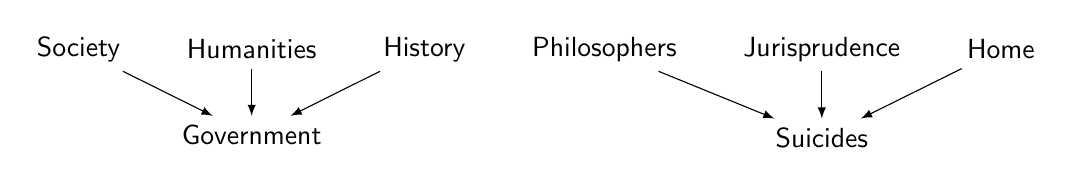
\begin{tikzpicture}[
            >=latex,
            node distance=0.6cm and 0.6cm
        ]
        \sffamily
        \node (society) {Society};
        \node[right=of society] (humanities) {Humanities};
        \node[right=of humanities] (history) {History};
        \node[below=of humanities] (government) {Government};
        \draw[->] (history) -- (government);
        \draw[->] (humanities) -- (government);
        \draw[->] (society) -- (government);

        \node[right=of history] (philosophers) {Philosophers};
        \node[right=of philosophers] (jurisprudence) {Jurisprudence};
        \node[right=of jurisprudence] (home) {Home};
        \node[below=of jurisprudence] (suicides) {Suicides};
        \draw[->] (philosophers) -- (suicides);
        \draw[->] (jurisprudence) -- (suicides);
        \draw[->] (home) -- (suicides);
    \end{tikzpicture}
    \caption{Example relations extracted by Hearst patterns.}
    \label{fig:hearst-example}
\end{figure}

\subsection{REBEL}

Instead of using hand-crafted patterns, one can use a more data-driven approach to relation extraction. The authors of REBEL~\cite{cabot2021rebel} frame relation extraction task as a neural translation problem: Given the source text (e.g., \texttt{A chihuahua is a kind of dog.}), the authors define the translation target in an invented ``relations language'' (e.g.,\texttt{<triplet> chihuahua <subj> dog <obj> subclass of}.). The author shares the trained model, REBEL-large\footnote{\url{https://huggingface.co/Babelscape/rebel-large}}, an encoder-decoder LLM based on BART-large \cite{lewis2019bart} trained to extract many types of relations from Wikipedia articles. Since we are only interested in taxonomic relations, I only use the ``subclass of'', ``instance of'', ``member of'' and ``part of'' relations that are extracted. Similar to Hearst patterns, I find that it fails to find many direct relations between ground truth concepts. The same low-rank smoothing technique is applied to give a higher recall.

\todo{Some qualitative results}

\subsection{Other baselines}

\paragraph{Memorisation}
Simply memorising the train graph is a surprisingly strong baseline due to the overlap between train and test graphs, especially for Wikipedia. The weight of each edge is given by the number of relevant subgraphs in which it appears.

\paragraph{Prompting}
We test the Zero/One/Three-shot performance of instruction-tuned LLMs on the subgraph modelling task described in \cref{sec:method:subgraph}. To obtain more comparable results, we use Mistral 7B Instruct v0.2, the instruction-tuned version of the base model of \name, as the LLM for our prompting baseline. For One-shot and Three-shot, random examples from the training set are sampled for each query. The output is parsed using regular expressions and results that do not match the patterns are discarded. I perform manual prompt engineering to optimise the model's responses by inspecting individual responses. The prompt template used is shown in \cref{fig:prompt-template} in Appendix~\ref{appendix:exp-details}.


\section{How to evaluate end-to-end OL?}  \label{sec:implementation:evaluation}

Since our problem setup is uncommon in existing literature, we also develop new evaluation methods. Ontology evaluation is a hard problem as there are no quantitative definitions of what constitutes a ``good ontology'' and metrics generally only capture one aspect of an ontology. We approach evaluation by treating the ground truth as a proxy for a good ontology and comparing the generated ontologies against the ground truth. This section describes how the ground truth is obtained and what metrics are used for measuring ontology similarity.

% Key points:
% \begin{enumerate}
%     \item Explain the goals of evaluation---what do we care about? Ans: Semantics and structure.
%     \item Suggest why end-to-end evaluation is hard: Large graph. Generally, a ``good ontology'' is ill-defined. Difficult to find one metric that describes all. Always trade-offs. No standard evaluation metric. 
%     \item How do we overcome this? 1. Use a ground truth ontology as a proxy for ``good ontology'' and measure how similar the generated ontology is to the ground truth. 2. Propose a series of evaluation metrics to capture various aspects of the generated output.
% \end{enumerate}

\subsection{Metrics}

Many existing methods for comparing ontologies rely on syntactic measures like string edit distance~\cite{Ehrig2005SimilarityFO} as a proxy for semantic similarity, or require every concept to be tagged with descriptions or documents for distributional semantics comparison~\cite{Zavitsanos2011GoldSE}. To obtain more robust and general evaluation results, we introduce a suite of similarity metrics that use modern methods like text embeddings~\cite{reimers-2019-sentence-bert}. Multiple metrics are used as they trade off between interpretability and comprehensiveness, and we aim to make them complementary by capturing different aspects of an ontology. We denote the ground truth ontology graph as $G = (V, E)$ and the generated graph as $G' = (V', E')$.

\textbf{Literal~F1 }
While literal text matching is unreliable, it is also the simplest and the most interpretable. We treat this metric as a reference metric for sanity check. The Literal~F1 metric~\cite{Kashyap2005TaxaMinerAE} is given by the harmonic mean of the precision and recall of the edges:
\[
    \text{Literal precision} = \frac{|E \cap E'|}{|E'|} \qquad
    \text{Literal recall} = \frac{|E \cap E'|}{|E|}
\]

\textbf{Fuzzy~F1 }
The Literal~F1 metric puts a strong emphasis on using the correct wording, while in practice, we are interested in evaluating the semantics of an ontology. For example, using a synonymous phrase for a concept should not be penalised. We utilise embeddings from a pretrained sentence transformer \cite{reimers-2019-sentence-bert} and use the cosine similarity of the embeddings to measure semantic similarity. Specifically, let $\nodesim(u, u') \in V \times V' \to [-1, 1]$ be the cosine similarity between the sentence embeddings for $u$ and $u'$. The Fuzzy~F1 score is obtained from the fuzzy precision and recall, defined as:
\begin{equation*}
    \begin{aligned}
        \text{Fuzzy precision} & = \frac{|
            \{(u', v') \in E' \mid \exists (u, v) \in E.
            \nodesim(u, u') > t \land \nodesim(v, v') > t
            \}
        |}{|E'|}                           \\
        \text{Fuzzy recall}    & = \frac{|
            \{(u, v) \in E \mid \exists (u', v') \in E'.
            \nodesim(u, u') > t \land \nodesim(v, v') > t
            \}
        |}{|E|}                            \\
    \end{aligned}
\end{equation*}
where $t$ is the matching threshold. We use all-MiniLM-L6-v2~\cite{wang2020minilm,reimers-2019-sentence-bert} as the embedding model, and choose $t$ as the median cosine similarity between the synonyms in WordNet~\cite{miller1995wordnet}, computed as~0.436.

\textbf{Continuous~F1 }
With fuzzy comparisons, the matches between the edges of the generated and the ground truth graph are no longer one-to-one. This is problematic: consider two graphs $A\!\rightarrow\!B$ and $B\!\leftarrow\!A\!\rightarrow\!B'$, where $B$ and $B'$ match fuzzily. Such graphs will achieve a perfect Fuzzy~F1 score yet they significantly differ. Additionally, we found that the previous metrics fail to provide a useful signal for hyperparameter tuning, particularly for our baselines where the generated graphs are poor. The Continuous~F1 metric solves these issues by computing the highest-scoring edge matching between the two graphs, where the similarity score between $(u, v)$ and $(u', v')$ is given by $\min(\nodesim(u, u'), \nodesim(v, v'))$. Obtaining such matching is equivalent to solving the linear assignment problem~\cite{martello1987linear}, which can be computed by the Hungarian algorithm~\cite{kuhn1955hungarian}. The Continuous~F1 score is obtained from the continuous precision and recall, given by:
\[
    \text{Continuous precision} = \frac{s_\text{cont}}{|E'|} \qquad
    \text{Continuous recall} = \frac{s_\text{cont}}{|E|}
\]
where $s_\text{cont}$ is the score achieved by the best edge matching.

\textbf{Graph~F1 }
Instead of individual edges, this metric aims to capture the wider structure of the two graphs. Intuitively, we want to know how concepts are related to their local neighbourhood. We do so by using simple graph convolutions~\cite{wu2019simplifying} with $K=2$ to compute graph-aware node embeddings after embedding each node with the pretrained embedder. Such embeddings in $G$ are compared against those in $G'$ by cosine similarity, and the highest-scoring node matching, similar to the Continuous~F1 metric, gives the graph similarity score. The Graph~F1 score is computed from the graph precision and recall, defined as:
\[
    \text{Graph precision} = \frac{s_\text{graph}}{|V'|} \qquad
    \text{Graph recall} = \frac{s_\text{graph}}{|V|}
\]
where $s_\text{graph}$ is the score achieved by the best node matching.

\textbf{Motif distance }
Taking inspiration from classical network analysis, we use \emph{network motifs}~\cite{milo2002network,shen2002network} to evaluate the structural integrity of the generated graphs. Network motifs are reoccurring subgraphs in a larger graph, most commonly 3-vertex subgraphs. They are typically indicative of the structural characteristics of the full graph. We define the motif distance as the 1-Wasserstein distance~\cite{Kantorovich1960MathematicalMO} between the distribution of all 3-vertex subgraphs in $G$ and $G'$.

\chapter{Evaluation}

In this chapter, we aim to answer our research questions:
\begin{enumerate}[leftmargin=*]
    \item Does \name produce better ontologies than traditional methods by subtask composition?
    \item Can \name be easily adapted to a new domain?
\end{enumerate}
Since our problem setup is uncommon in existing literature, we also develop new evaluation methods. Evaluating a quality of an ontolgoy is a hard problem as there are no quantitative definitions of what constitutes a ``good ontology'', and metrics generally only capture one aspect (e.g., structure but not semantics) of an ontology. We approach evaluation by treating the ground truth as a proxy for a good ontology, and comparing the generated ontologies against the ground truth.

In \cref{sec:metrics}, we introduce new metrics that are more robust for measuring ontology similarity. We design our experiments to answer the research questions in \cref{sec:experiments}, and present the results in \cref{sec:results}. We show that \name outperforms all of our baselines and can be easily adapted to a new domain using a small number of training samples, demonstrating the potential of \name for end-to-end OL.

\section{Metrics}  \label{sec:metrics}

Many existing methods for comparing ontologies rely on syntactic measures like string edit distance~\cite{Ehrig2005SimilarityFO} as a proxy for semantic similarity, or require every concept to be tagged with descriptions or documents for distributional semantics comparison~\cite{Zavitsanos2011GoldSE}. To obtain more robust and general evaluation results, we introduce a suite of similarity metrics that use modern methods like text embeddings~\cite{reimers-2019-sentence-bert}. Multiple metrics are used as they trade off between interpretability and comprehensiveness, and we aim to make them complementary by capturing different aspects of an ontology. In this section, we denote the ground truth ontology graph as $G = (V, E)$ and the generated graph as $G' = (V', E')$.

\paragraph{Literal~F1}
While literal text matching is unreliable, it is also the simplest and the most interpretable. We treat this metric as a reference metric for sanity check. The Literal~F1 metric~\cite{Kashyap2005TaxaMinerAE} is given by the harmonic mean of the precision and recall of the edges:
\[
    P_{\text{literal}} = \frac{|E \cap E'|}{|E'|} \qquad
    R_{\text{literal}} = \frac{|E \cap E'|}{|E|} \qquad
    \text{Literal~F1} = \left(\frac{1}{P_{\text{literal}}} + \frac{1}{R_{\text{literal}}}\right)^{-1}
\]

\paragraph{Fuzzy~F1}
The Literal~F1 metric puts a strong emphasis on using the correct wording, while in practice, we are interested in evaluating the semantics of an ontology. For example, using a synonymous phrase for a concept should not be penalised. The current state-of-the-art for semantic textual similarity tasks are sentence transformers \cite{reimers-2019-sentence-bert,jiang2022improved,jiang2019smart}. On a high level, a sentence transformer is an embedding function $f: \text{string} \to \mathbb{R}^d$ that maps a string to a $d$-dimensional vector space such that semantically similar strings are close in the vector space, usually measured by cosine similarity:
\[
    \nodesim(u, u') = \frac{f(u) \cdot f(u')}{\|f(u)\| \|f(u')\|}
\]
We consider two nodes $u$ and $u'$ as a fuzzy match if $\nodesim(u, u') > t$, where $t$ is a threshold, chosen to be the median cosine similarity between the synonyms in WordNet~\cite{miller1995wordnet} (computed as 0.436). Two edges $(u, v)$ and $(u', v')$ are a fuzzy match if both $u$ and $v$ are fuzzy matches with $u'$ and $v'$ respectively. The Fuzzy~F1 score is given by the precision and recall of the fuzzy matches:
\begin{equation*}
    \begin{aligned}
        P_{\text{fuzzy}} & = \frac{|
            \{(u', v') \in E' \mid \exists (u, v) \in E.
            \nodesim(u, u') > t \land \nodesim(v, v') > t
            \}
        |}{|E'|}                                                                                       \\
        R_{\text{fuzzy}} & = \frac{|
            \{(u, v) \in E \mid \exists (u', v') \in E'.
            \nodesim(u, u') > t \land \nodesim(v, v') > t
            \}
        |}{|E|}                                                                                        \\
        \text{Fuzzy~F1}  & = \left(\frac{1}{P_{\text{fuzzy}}} + \frac{1}{R_{\text{fuzzy}}}\right)^{-1}
    \end{aligned}
\end{equation*}
The Fuzzy~F1 metric can be seen as a generalisation of the Literal~F1 metric: we recover the Literal~F1 metric if $t = 1$. We use all-MiniLM-L6-v2~\cite{wang2020minilm,reimers-2019-sentence-bert} as the embedding model.

\paragraph{Continuous~F1}
With fuzzy comparisons, the matches between the edges of the generated and the ground truth graph are no longer one-to-one. This is problematic when there are repetitive elements:
\begin{figure}[H]
    \centering
    \begin{tikzpicture}[>=latex]
        \sffamily
        \newcommand{\dist}{1.5cm}
        \node (A1) {A};
        \node (B1) at ($(A1) + (0, -\dist)$) {B};
        \draw[->] (A1) -- (B1);

        \node (A2) at ($(A1) + (2.5, 0)$) {A};
        \node (B2) at ($(A2) + (-0.8, -\dist)$) {B};
        \node (B2') at ($(A2) + (0.8, -\dist)$) {B'};
        \draw[->] (A2) -- (B2);
        \draw[->] (A2) -- (B2');
    \end{tikzpicture}
\end{figure}
\vspace{-1em}
where $B$ and $B'$ match fuzzily. This pair of graphs achieves a perfect Fuzzy~F1 score, yet they are clearly different. Additionally, we found that the discrete nature of Fuzzy F1 makes it unable to provide useful signals for hyperparameter tuning, particularly for our baselines where the generated graphs are poor. The Continuous~F1 metric solves these issues by computing the highest-scoring edge matching between the two graphs, where the similarity score between $(u, v)$ and $(u', v')$ is given by $\min(\nodesim(u, u'), \nodesim(v, v'))$. We choose to use $\min(\nodesim(u, u'), \nodesim(v, v'))$ as the similarity score to ensure that only edges where both nodes partially match (i.e. cosine similarity $> 0$) can contribute to the total matching score. Obtaining such matching is equivalent to solving the linear assignment problem~\cite{martello1987linear}, which can be computed by the Hungarian algorithm~\cite{kuhn1955hungarian}. Given the score $s_{\text{cout}}$ achieved by the best edge matching, the Continuous~F1 score is obtained from the continuous precision and recall, given by:
\[
    P_{\text{cont}} = \frac{s_{\text{cout}}}{|E'|} \qquad
    R_{\text{cont}} = \frac{s_{\text{cout}}}{|E|} \qquad
    \text{Continuous~F1} = \left(\frac{1}{P_{\text{cont}}} + \frac{1}{R_{\text{cont}}}\right)^{-1}
\]

\paragraph{Graph~F1}
Instead of comparing individual edges, this metric aims to capture the wider structure of the two graphs. Intuitively, we want to know how concepts are related to their local neighbourhood. A well known method for capturing graph structure in vectors is node embeddings, as discussed in \cref{sec:node-embeddings}. Concretely, we use simple graph convolutions \cite{wu2019simplifying} with identity weights and $K=2$ as a parameter-free method to compute graph-aware node representations after embedding each node with the pretrained embedder. Such embeddings in $G$ are compared against those in $G'$ by cosine similarity, and the highest-scoring node matching, similar to the Continuous~F1 metric, gives the graph similarity score $s_{\text{graph}}$. The Graph~F1 score is computed from the graph precision and recall, defined as:
\[
    P_{\text{graph}} = \frac{s_{\text{graph}}}{|V'|} \qquad
    R_{\text{graph}} = \frac{s_{\text{graph}}}{|V|} \qquad
    \text{Graph~F1} = \left(\frac{1}{P_{\text{graph}}} + \frac{1}{R_{\text{graph}}}\right)^{-1}
\]

\paragraph{Motif distance}
Taking inspiration from classical network analysis, we use \emph{network motifs}~\cite{milo2002network,shen2002network} to evaluate the structural integrity of the generated graphs. Network motifs are reoccurring subgraphs in a larger graph, most commonly 3-vertex subgraphs. They are typically indicative of the structural characteristics of the full graph. We define the motif distance as the 1-Wasserstein distance~\cite{Kantorovich1960MathematicalMO} between the distribution of all 3-vertex subgraphs in $G$ and $G'$.


\section{Experiments}  \label{sec:experiments}

We design our experiments to answer the following research questions:
\begin{enumerate}
    \item Does \name produce better ontologies than traditional methods by subtask composition?
    \item Can \name be easily adapted to a new domain?
\end{enumerate}
We approach the questions by training \name on the Wikipedia dataset and further transfer the model to arXiv with a small number of arXiv samples. As baselines, we use two relation extraction methods, Hearst patterns \cite{hearst1998automated,roller2018hearst} and REBEL \cite{cabot2021rebel}. Relation extraction depends on successful concept discovery to produce high-quality ontologies. To estimate a ceiling to such baselines, \emph{we give the baselines a substantial advantage} by providing them with the ground truth concepts in the test graph. The results show that even with such an advantage, \name outperforms the baselines on many metrics, demonstrating the potential of \name for end-to-end OL.

\subsection{Implementation details}  \label{sec:implementation}


The model is trained on the Wikipedia dataset for two epochs with Adam. During inference, the outputs are generated with temperature 0.1 and nucleus sampling~\cite{holtzman2019curious} top-$p$ of 0.9. We include a finetuning baseline without the masked loss objective, denoted as Finetune. To adapt \name for arXiv, we further finetune the model on 2048 document-subgraph pairs from arXiv. We initialise new low-rank adaptors and train until the loss stops improving on the validation set. We name these models \name (transfer) and Finetune (transfer) for training with and without the masked loss objective, respectively. Full details for the Wikipedia and arXiv experiments can be found in~\cref{appendix:training-details}.


The hyperparameters for the post-processing steps are tuned by grid search on the validation set. We sweep over $\alpha \in 1 - \text{geomspace}(1 / |E_\text{raw}|, 1, 21)$ and $\beta \in \text{geomspace}(0.1, 1, 21) - 0.1$ and use the values that maximise Continuous~F1. For Wikipedia, we choose the subgraph modelling path length $N=4$ as it is the smallest $N$ such that almost all edges ($>99\%$) occur in at least one relevant subgraph. Such criterion is used since smaller $N$ results in smaller subgraphs, which we expect to be easier to model accurately. We choose $N=3$ for arXiv for the same reason.


\section{Results}  \label{sec:results}

{
\addtolength{\tabcolsep}{-0.2em}
\begin{table}[t!]
\caption{Evaluation metrics of \name and baselines on Wikipedia and arXiv. \name performs particularly well in modelling semantics, and remains competitive syntactically and structurally.}
\label{table:metrics}
\centering
\begin{small}
\begin{tabularx}{\linewidth}{l l X X X X l}
\toprule
Dataset & Method & Literal F1 $\uparrow$ & Fuzzy F1 $\uparrow$ & Cont. F1 $\uparrow$ & Graph F1 $\uparrow$ & Motif Dist. $\downarrow$ \\
\midrule
\multirow[t]{8}{*}{Wikipedia} & Memorisation & \textbf{0.134} & 0.837 & 0.314 & 0.419 & 0.063 \\
 & Hearst & 0.003 & 0.538 & 0.350 & 0.544 & 0.163 \\
 & Rebel & 0.004 & 0.624 & 0.356 & 0.072 & 0.132 \\
 & Zero-shot & 0.007 & 0.871 & 0.455 & 0.639 & 0.341 \\
 & One-shot & 0.031 & 0.888 & 0.477 & 0.610 & 0.314 \\
 & Three-shot & 0.031 & 0.880 & 0.475 & 0.622 & 0.354 \\
 & Finetune & 0.124 & 0.884 & 0.470 & 0.588 & \textbf{0.050} \\
 & \textbf{\name} & 0.093 & \textbf{0.915} & \textbf{0.500} & \textbf{0.644} & 0.080 \\
\midrule
\multirow[t]{8}{*}{arXiv} & Memorisation & 0.000 & 0.207 & 0.257 & 0.525 & \textbf{0.037} \\
 & Hearst & 0.000 & 0.000 & 0.151 & 0.553 & 0.098 \\
 & Rebel & 0.000 & 0.060 & 0.281 & 0.546 & 0.088 \\
 & Zero-shot & 0.025 & 0.450 & 0.237 & 0.414 & 0.145 \\
 & One-shot & \textbf{0.072} & 0.460 & 0.290 & 0.433 & 0.293 \\
 & Three-shot & 0.051 & 0.405 & 0.212 & 0.385 & 0.124 \\
 % & Finetune & 0.000 & 0.196 & 0.228 & 0.359 & 0.606 \\
 % & Finetune masked & 0.000 & 0.097 & 0.169 & 0.385 & 0.413 \\
 & Finetune (transfer) & 0.000 & 0.440 & 0.225 & 0.441 & 0.148 \\
& \textbf{\name} (transfer) & 0.040 & \textbf{0.570} & \textbf{0.357} & \textbf{0.633} & 0.097 \\
\bottomrule
\end{tabularx}
\vspace*{-4mm}
\end{small}
\end{table}
}

We first evaluate whether \name can accurately create ontologies with many concepts and relations, such as the Wikipedia categories. Computationally, \name required 12 A100-hours for training and 7 A100-hours for inference to generate an ontology for Wikipedia. This is a modest cost in current standards, which demonstrates the scalability of \name for real-world problems.
In terms of performance, \name produces the most semantically accurate ontology in comparison to our baselines as presented in \cref{table:metrics}. Across all of Fuzzy~F1, Continuous~F1 and Graph~F1, we observe the trend that \name scores the best, followed by Finetune and Prompting, and lastly Hearst and REBEL. This is surprising, as it suggests that the combination of LLMs with our subgraph modelling framework is a sufficiently strong inductive bias for LLMs to outperform traditional methods even without finetuning. However, prompting alone is not sufficient to build high-quality ontologies.
On the Motif Distance metric, prompting methods score poorly at 0.314--0.354 in comparison to 0.050 and 0.080 for Finetune and \name respectively. This shows that using LLMs out-of-the-box for subgraph modelling results in poor structural integrity, though this issue is solved by finetuning.
Qualitatively, we observe that \name can adhere to the clear, explicit naming style of Wikipedia, even on unseen topics in the test set. For example, it generates ``Mathematical categories'' and ``Groups (mathematics)'' under the parent concept ``Mathematical structures'' to distinguish from the natural language sense of categories and groups (\cref{fig:ollm-wiki-samples-math}). Such style is not learned by the prompting baselines: Three-shot generated ``Elections $\to$ France'', while it most likely meant ``Elections $\to$ Elections in France'' (\cref{fig:3shot-wiki-samples-election}). More sample outputs are shown in \cref{appendix:viz-wiki}.

The arXiv task differs from the Wikipedia task as it has much fewer relations, and there is even less overlap between the train and test split. This imposes a great challenge on Finetune and \name as they need to generalise with a limited diversity of training samples. Despite such constraints, \name is substantially better than other methods in modelling the semantics of the test graph.
On the Fuzzy~F1, Continuous~F1, and Graph~F1 metrics, \name performs the best among all methods with 0.570, 0.357, and 0.633, significantly higher than the next-best of 0.460, 0.290 and 0.546 respectively.
Inspecting the generated ontologies (\cref{appendix:viz-arxiv}), we observe that prompting baselines tend to produce repetitive concepts such as ``Machine Learning and Artificial Intelligence'' and ''Artificial Intelligence and Machine Learning'' (\cref{fig:3shot-arxiv}), while Hearst and REBEL put almost all concepts under the same parent concept(s) (\cref{fig:hearst-arxiv,fig:rebel-arxiv}).
We also found that \name's output for arXiv contains concepts from Wikipedia, but restructured in a way that fits the arXiv ontology. For example, ``Life sciences'' and ``Biological evolution'' appear in the Wikipedia training set under the same parent category ``Life'' with no direct links between them. On the generated graph for arXiv, ``Life sciences'' is instead promoted to one of the top-level concepts with ``Biological Evolution'' as one of its children, which better fits the ``fields of science'' style of the arXiv ontology (\cref{fig:ollm-arxiv}). This demonstrates that \name can adapt to produce a new type of ontology by restructuring its learned concepts, all using just a small number of training samples.

In summary, \name scores the best or is competitive across all metrics in both tasks, with the notable exception of the Literal~F1 metric. We attribute this to the fact that Literal~F1 is sensitive to factors like casing and choice of words, and generally only measures syntactic similarity. For example, we see that a suboptimal baseline like Memorisation scores the best on this metric with 0.134 on the Wikipedia task. This reflects that syntactic similarity generally does not entail semantic similarity so syntax-based metrics should not be used as stand-alone measures for ontology quality.


\chapter{Conclusion}

\section{Achievements}

This project is successful and has met all of its project goals (\cref{chap:introduction}). Our contributions are in two main directions. First, we propose and study the novel task of end-to-end OL, where the only goal is to build a high-quality ontology from scratch. To facilitate this paradigm shift, we contribute the foundational elements for a new task, including two new datasets (Wikipedia and arXiv), a series of baselines (Hearst, REBEL, and Prompting), and a novel suite of evaluation metrics (Fuzzy F1, Continuous F1, Graph F1, and Motif Distance). Second, we introduce \name, a general, scalable, and performant method that leverages LLMs to build ontologies from scratch. \name outperforms traditional subtask composition methods in reconstructing the Wikipedia categories, and can be transferred to build ontologies for arXiv after finetuning on a small number of examples. In the process, we overcome several challenges:
\begin{enumerate}
    \item \textbf{Overfitting}: Through in-depth analysis of the per-token test loss of a naively finetuned LLM, we discover the root cause of poor generalisation to be overfitting to high-frequency concepts. With this insight, we propose a custom regulariser tailored for our problem setup that reweights each concept based on its frequency of occurrence, which substantially improves generalisation.
    \item \textbf{Lack of references}: The lack of prior works on end-to-end OL means that there are no standard approaches to many components of the project, such as how to create train-test splits for ontologies. This leaves us with numerous design decisions, which we approach by first principles and draw as many connections to other areas of machine learning as possible, including classical graph analysis, graph neural networks, text embeddings, multitask learning, and transfer learning.
\end{enumerate}


\section{Limitations and future work}

% More types of inputs
% More types of relations
% Strict outputs (transitivity constraints)
% More niche domains
There are several factors that we did not address as they are beyond the scope of this project, but are interesting directions for future work:
\begin{enumerate}
    \item \textbf{More complex ontologies}: We only study and evaluate the construction of ontologies with only concepts and taxonomic relations. A potential approach to extend \name to produce non-taxonomic relations is to add tags indicating the relation type to each edge when linearising the subgraphs for sequence modelling. New evaluation metrics might also be required to handle multiple types of relations.
    \item \textbf{Transitivity constraints}: The taxonomic relations in the generated ontologies are not necessarily transitive due to the possible existence of cycles. We relaxed the transitivity constraints for simplicity, though the formal semantics may be important for some applications. This is a common problem for many OL methods and there are existing works on cycle removal algorithms for cleaning hierarchies~\cite{sun2017breaking,zesch2007analysis}.
    \item \textbf{Data contamination}: We were unable to fully control for data leakage as the pretraining dataset of Mistral 7B is not publicly known. We do, however, observe that the generated ontologies are sufficiently different from the ground truth, indicating that \name is not directly remembering samples from its pretraining stage. One can further investigate the impact of pretraining data contamination by using base models such as OLMo \cite{OLMo} that has open-source pretraining data.
    \item \textbf{Other types of inputs}: We only use the text of the Wikipedia and arXiv articles as input to the model, both of which covers concepts that are quite general. Future work should investigate whether the approach is also applicable to more niche domains, such as protein types or chemical compounds. Using LLMs as the backbone for subgraph modelling opens up possibilities to handle other kinds of inputs. For example, one may generate ontologies from corpora with images using vision language models~\cite{donahue2015long}.
\end{enumerate}

\section{Final remarks}

This project is an original attempt at studying OL in an end-to-end fashion. We believe the success of \name is a testament to the potential of this end-to-end paradigm, and we hope that this work will inspire more research in this direction. Future work can benefit from the methodology used in this project, such as the dataset, the train-test split strategy, and the evaluation metrics that we introduced. Our result is also easily applicable to a practical setting. We release our model \name in hopes that practitioners can use it to build ontologies in the real world right now with minimal manual effort.

\label{lastcontentpage} % end page count here

%TC:ignore 
\bibliographystyle{plainnat}
\bibliography{references}

\appendix

\chapter{Technical details, proofs, etc.}

Appendices are for optional materials that is not essential to
understanding the work, and that the examiners are not expected to
read, but that will be of value to readers interested in additional,
in-depth technical detail.

\section{Lorem ipsum}

% Some traditional fake Latin prose for calibrating words/page
Lorem ipsum dolor sit amet, consetetur sadipscing elitr, sed diam
nonumy eirmod tempor invidunt ut labore et dolore magna aliquyam erat,
sed diam voluptua. At vero eos et accusam et justo duo dolores et ea
rebum. Stet clita kasd gubergren, no sea takimata sanctus est Lorem
ipsum dolor sit amet. Lorem ipsum dolor sit amet, consetetur
sadipscing elitr, sed diam nonumy eirmod tempor invidunt ut labore et
dolore magna aliquyam erat, sed diam voluptua. At vero eos et accusam
et justo duo dolores et ea rebum. Stet clita kasd gubergren, no sea
takimata sanctus est Lorem ipsum dolor sit amet. Lorem ipsum dolor sit
amet, consetetur sadipscing elitr, sed diam nonumy eirmod tempor
invidunt ut labore et dolore magna aliquyam erat, sed diam voluptua.
At vero eos et accusam et justo duo dolores et ea rebum. Stet clita
kasd gubergren, no sea takimata sanctus est Lorem ipsum dolor sit
amet.

\section{Homo sapiens non urinat in ventum}
Duis autem vel eum iriure dolor in hendrerit in vulputate velit esse
molestie consequat, vel illum dolore eu feugiat nulla facilisis at
vero eros et accumsan et iusto odio dignissim qui blandit praesent
luptatum zzril delenit augue duis dolore te feugait nulla facilisi.
Lorem ipsum dolor sit amet, consectetuer adipiscing elit, sed diam
nonummy nibh euismod tincidunt ut laoreet dolore magna aliquam erat
volutpat.

%TC:endignore 

\label{lastpage}
\end{document}
